\chapter{SYSTEM ANALYSIS AND DESIGN}
\section{System Analysis}
The project is following a structured approach that utilizes the Rapid Application Development (RAD) methodology. This approach segments the project into smaller, manageable components, allowing for incremental progress through iterative development. Individual modules are developed and integrated progressively, focusing on delivering and refining smaller segments. This method ensures continuous improvement and alignment with the overall goals while effectively managing the project through ongoing feedback and adjustments.
\subsection{Requirement Analysis}
Requirement analysis is a critical phase in the software development lifecycle that focuses on understanding and documenting the needs and expectations of stakeholders. This process involves gathering detailed information about what users require from a system, which includes identifying functional requirements (what the system should do), non-functional requirements (how the system should perform), and constraints (limitations or restrictions). The goal is to create a comprehensive and clear specification that guides the development team in designing and implementing the system. Effective requirement analysis ensures that the final product aligns with user needs and business objectives, reduces the risk of project failure, and facilitates efficient communication among stakeholders. By thoroughly analyzing requirements, teams can address potential issues early, prioritize features, and ensure a smoother development process.
\subsubsection{Functional Requirements}The functional requirements of LabXplorerX are mentioned below:
\begin{itemize}
    \item \textbf{User Profiles:}  
    LabXplorerX allows children and teachers to create personalized profiles for managing their activity within the platform. Users can log in with unique credentials and update their profiles with avatars and educational interests. The profile section displays only the user's own comments and interactions within the platform, along with a list of their favorited capsules. This streamlined approach helps users easily track their contributions and revisit their most valued content.

    \item \textbf{Interactive Virtual Simulations:} LabXplorerX offers a range of interactive virtual simulations, including Basic Electronics, Basic Chemistry, Basic Astronomy, and an Online Coding Environment. These simulations provide immersive experiences where users can engage in hands-on activities, such as manipulating virtual equipment and conducting experiments. By integrating interactive animations and real-world scenarios, LabXplorerX facilitates experiential learning, allowing users to explore scientific principles and phenomena in a dynamic digital environment.

    \item \textbf{Capsule Tools:}  
    In LabXplorerX, only administrators have the ability to create educational capsules, quizzes, and simulation links. They can design capsules with interactive quizzes, organize educational content, and provide structured learning paths for students. However, the creation and development of new simulations are restricted to developers, ensuring that complex interactive simulations are handled by technical experts while allowing administrators to manage and assign tasks within the platform.
    

    \item \textbf{Comments and Favourites for Learning Capsules:}  
    LabXplorerX provides a comments section for each learning capsule, allowing students and teachers to leave feedback, ask questions, or share insights directly related to the content. Users can engage with one another by commenting on specific capsules. Additionally, the platform supports a "favourites" feature, enabling users to bookmark and easily revisit their preferred capsules, enhancing their personalized learning experience.


    \item \textbf{Quizzes and Learning Capsules:} LabXplorerX integrates quizzes and learning capsules to reinforce knowledge and assess comprehension. Quizzes are designed to evaluate understanding of concepts covered in simulations, while learning capsules provide bite-sized, focused content on specific topics. These features help consolidate learning and provide instant feedback.

    \item \textbf{Admin Dashboard:}  
    The admin dashboard in LabXplorerX provides a centralized interface for managing user accounts, monitoring platform usage, and overseeing system performance. Administrators have the ability to perform full CRUD (Create, Read, Update, Delete) operations on quizzes and capsules, ensuring content is up-to-date and relevant. They can also add simulation links to capsules, making it easier to integrate simulations into the learning experience, while maintaining control over the platform's content and functionality.

\end{itemize}

\begin{figure}[H]
    \centering
     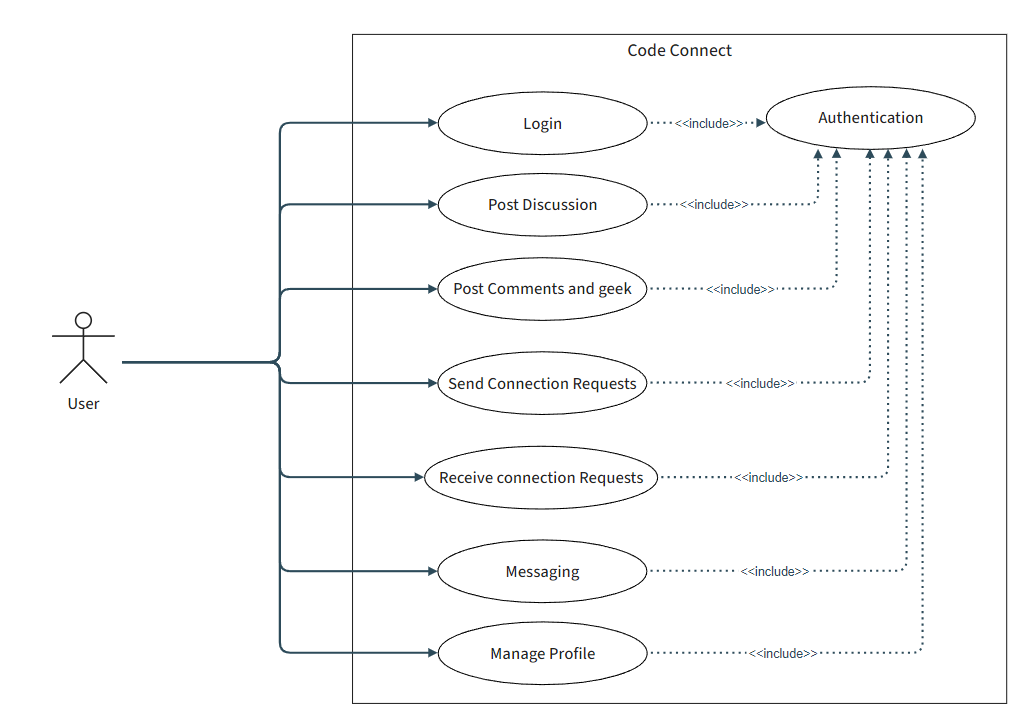
\includegraphics[height = 12cm]{Diagrams/use_case.png}
     \caption{Use Case Diagram}
 \end{figure}

\subsubsection{Nonfunctional Requirements}
The nonfunctional requirements of LabXplorerX are mentioned below:
\begin{itemize}
    \item \textbf{Performance Enhancement:} The focus on performance involves optimizing the platform to handle high user loads and complex simulations efficiently. This includes minimizing reliance on external frameworks and ensuring smooth and responsive interactions.
    \item \textbf{Authentication Security:} Security is a paramount concern. To enhance the platform’s security, advanced authentication algorithms, particularly focusing on hashing techniques within the backend environment, have been implemented. This ensures that user authentication data is stored and managed in a highly secure manner.
    \item \textbf{Better UX Design:} User experience is central to the project’s success. The emphasis on better UX design means that every aspect of the platform’s interface, from navigation to interaction, will be meticulously crafted to ensure a seamless and intuitive experience. This design approach caters not only to experienced users but also to newcomers, ensuring that all users can effortlessly navigate and engage with the platform.
    \item \textbf{Responsive Design:}  
    Recognizing the diverse range of devices and browsers used by users, the platform features a responsive design that ensures optimal adaptation across different screen sizes for most interface elements. This means that users can effectively access and interact with the platform whether they are using a desktop computer, tablet, or smartphone. However, it's important to note that the simulations are not responsive and are limited to desktop use. This approach guarantees a consistent and satisfying experience on various devices for general content, while simulations remain optimized for desktop environments.

\end{itemize}
\section{Feasibility Analysis}
A feasibility study is a systematic and structured analysis conducted to determine the viability and practicality of a proposed project plan. It serves as an evaluation tool to assess whether the project can be successfully implemented and if it aligns with the organization's goals and objectives. It involves gathering and analyzing relevant information to determine if the project is technically feasible, operationally feasible, economically feasible, and scheduling feasible.
\subsection{Economical Feasibility}
The development of the web application will utilize a range of free and open-source software development tools. For the frontend, React, a popular JavaScript library for building dynamic and interactive user interfaces, will be used. On the backend, Express, a minimal and flexible Node.js web application framework, will handle server-side logic and HTTP requests. PostgreSQL, an open-source relational database management system known for its reliability and performance, will be employed for database management. Interactive simulations will be created using Phaser, a robust HTML5 game framework, while Unity, a powerful cross-platform game engine, will be used for more complex simulations and 3D elements. Additionally, funds will be allocated for economical server hosting to ensure the application remains accessible to users while managing costs effectively.
\subsection{Operational Feasibility}
LabXplorerX prioritizes operational feasibility through a user-centric design approach, emphasizing simplicity and ease of use. The system is highly interactive, enabling both students and educators to navigate effortlessly without requiring extensive technical knowledge. The user interface (UI) features a clean layout and intuitive controls, ensuring a seamless experience when accessing virtual environments and educational resources. By minimizing the need for extensive training and reducing potential barriers to adoption, LabXplorerX enhances user acceptance and engagement. The straightforward design promotes effective use of the app's features, supports educational activities, and fosters a positive user experience.
\subsection{Technical Feasibility}
Combining Express.js with React and PostgreSQL offers a robust and scalable solution for developing modern applications. Express.js, built on Node.js, provides an efficient backend framework for creating RESTful APIs and managing server-side logic. PostgreSQL, known for its reliability and advanced data management features, serves as a solid foundation for secure and efficient data storage and querying. On the frontend, React facilitates the creation of responsive and visually appealing applications across multiple platforms using a single codebase. This stack leverages the strengths of each technology: Express.js for backend scalability and API development, PostgreSQL for comprehensive data handling, and React for seamless and dynamic UI development. Supported by active communities and extensive documentation, this combination ensures ample technical support, resources, and flexibility for both deployment and maintenance, making it an ideal choice for delivering modern, interactive applications.
\section{Structured System Modelling }
Structured system modeling is a methodical approach used to design complex systems by decomposing them into manageable components and utilizing formal diagrams and tools. This approach aids in clearly defining system requirements, workflows, and interactions. By breaking down a system into its constituent parts, structured system modeling facilitates a thorough understanding of its structure and behavior. The use of formal diagrams and tools ensures that all aspects of the system are documented and analyzed systematically, which enhances clarity, communication, and accuracy throughout the design process. This methodical approach supports the creation of well-organized and efficient systems, improving overall design quality and project outcomes.
\newpage
\subsection{Process Modeling}
Processing Modeling visually represent the flow of data within a system, showing how inputs are processed into outputs. They help in understanding the system's functionality and data movement, aiding in the design and analysis of processes.
\begin{figure}[H]
    \centering
        
\includegraphics[height = 18cm]{Diagrams/ProcessModelling.png}
    \caption{Process Model: Logical DFD}
\end{figure}
\newpage
\newpage
\subsection{Data Modelling(ER-Diagram)}
The Entity-Relationship (ER) Diagram is primarily used to design a database schema. The ER diagram provided below facilitates the creation of a database in SQL by clearly illustrating the entities, their attributes, and the relationships between them. This visual representation helps in structuring the database effectively, ensuring that all necessary data elements and their interconnections are accounted for.
\section*{Entities and Attributes}
\begin{itemize}
    \item \textbf{Users}
    \begin{itemize}
        \item \texttt{id}: Unique identifier for the user.
        \item \texttt{username}: The name of the user.
        \item \texttt{email}: Email of the user.
        \item \texttt{password}: Password for user authentication.
        \item \texttt{email\_verification\_token}: Token to verify the email.
        \item \texttt{email\_verified}: Status indicating whether the user's email is verified.
    \end{itemize}
    
    \item \textbf{Capsules}
    \begin{itemize}
        \item \texttt{id}: Unique identifier for the capsule.
        \item \texttt{title}: Title of the capsule.
        \item \texttt{description}: Description of the capsule.
        \item \texttt{thumbnail}: Image representing the capsule.
        \item \texttt{images}: Additional images related to the capsule.
        \item \texttt{pdf}: PDF documents associated with the capsule.
        \item \texttt{category}: The category to which the capsule belongs.
        \item \texttt{author\_id}: Reference to the user who created the capsule.
    \end{itemize}
    
    \item \textbf{Simulations}
    \begin{itemize}
        \item \texttt{id}: Unique identifier for the simulation.
        \item \texttt{title}: Title of the simulation.
        \item \texttt{description}: Description of the simulation.
        \item \texttt{link}: URL or reference to the simulation.
        \item \texttt{category}: The category of the simulation.
    \end{itemize}
    
    \item \textbf{Comments}
    \begin{itemize}
        \item \texttt{comment\_id}: Unique identifier for the comment.
        \item \texttt{comment\_text}: The text of the comment.
        \item \texttt{user\_id}: Reference to the user who made the comment.
        \item \texttt{capsule\_id}: Reference to the capsule that was commented on.
    \end{itemize}
    
    \item \textbf{Quiz}
    \begin{itemize}
        \item \texttt{quiz\_id}: Unique identifier for the quiz.
        \item \texttt{title}: Title of the quiz.
        \item \texttt{category}: The category of the quiz.
        \item \texttt{capsule\_id}: Reference to the capsule related to the quiz.
    \end{itemize}
    \item \textbf{Options}
    \begin{itemize}
        \item \texttt{option\_id}: Unique identifier for the option.
        \item \texttt{option\_text}: Text of the quiz option.
        \item \texttt{is\_correct}: Boolean indicating if the option is correct.
        \item \texttt{quiz\_id}: Reference to the quiz.
    \end{itemize}
    
    \item \textbf{Favorites}
    \begin{itemize}
        \item \texttt{user\_id}: Reference to the user.
        \item \texttt{capsule\_id}: Reference to the capsule marked as a favorite.
    \end{itemize}
\end{itemize}
\begin{figure}[H]
    \centering
    \rotatebox{90}{
        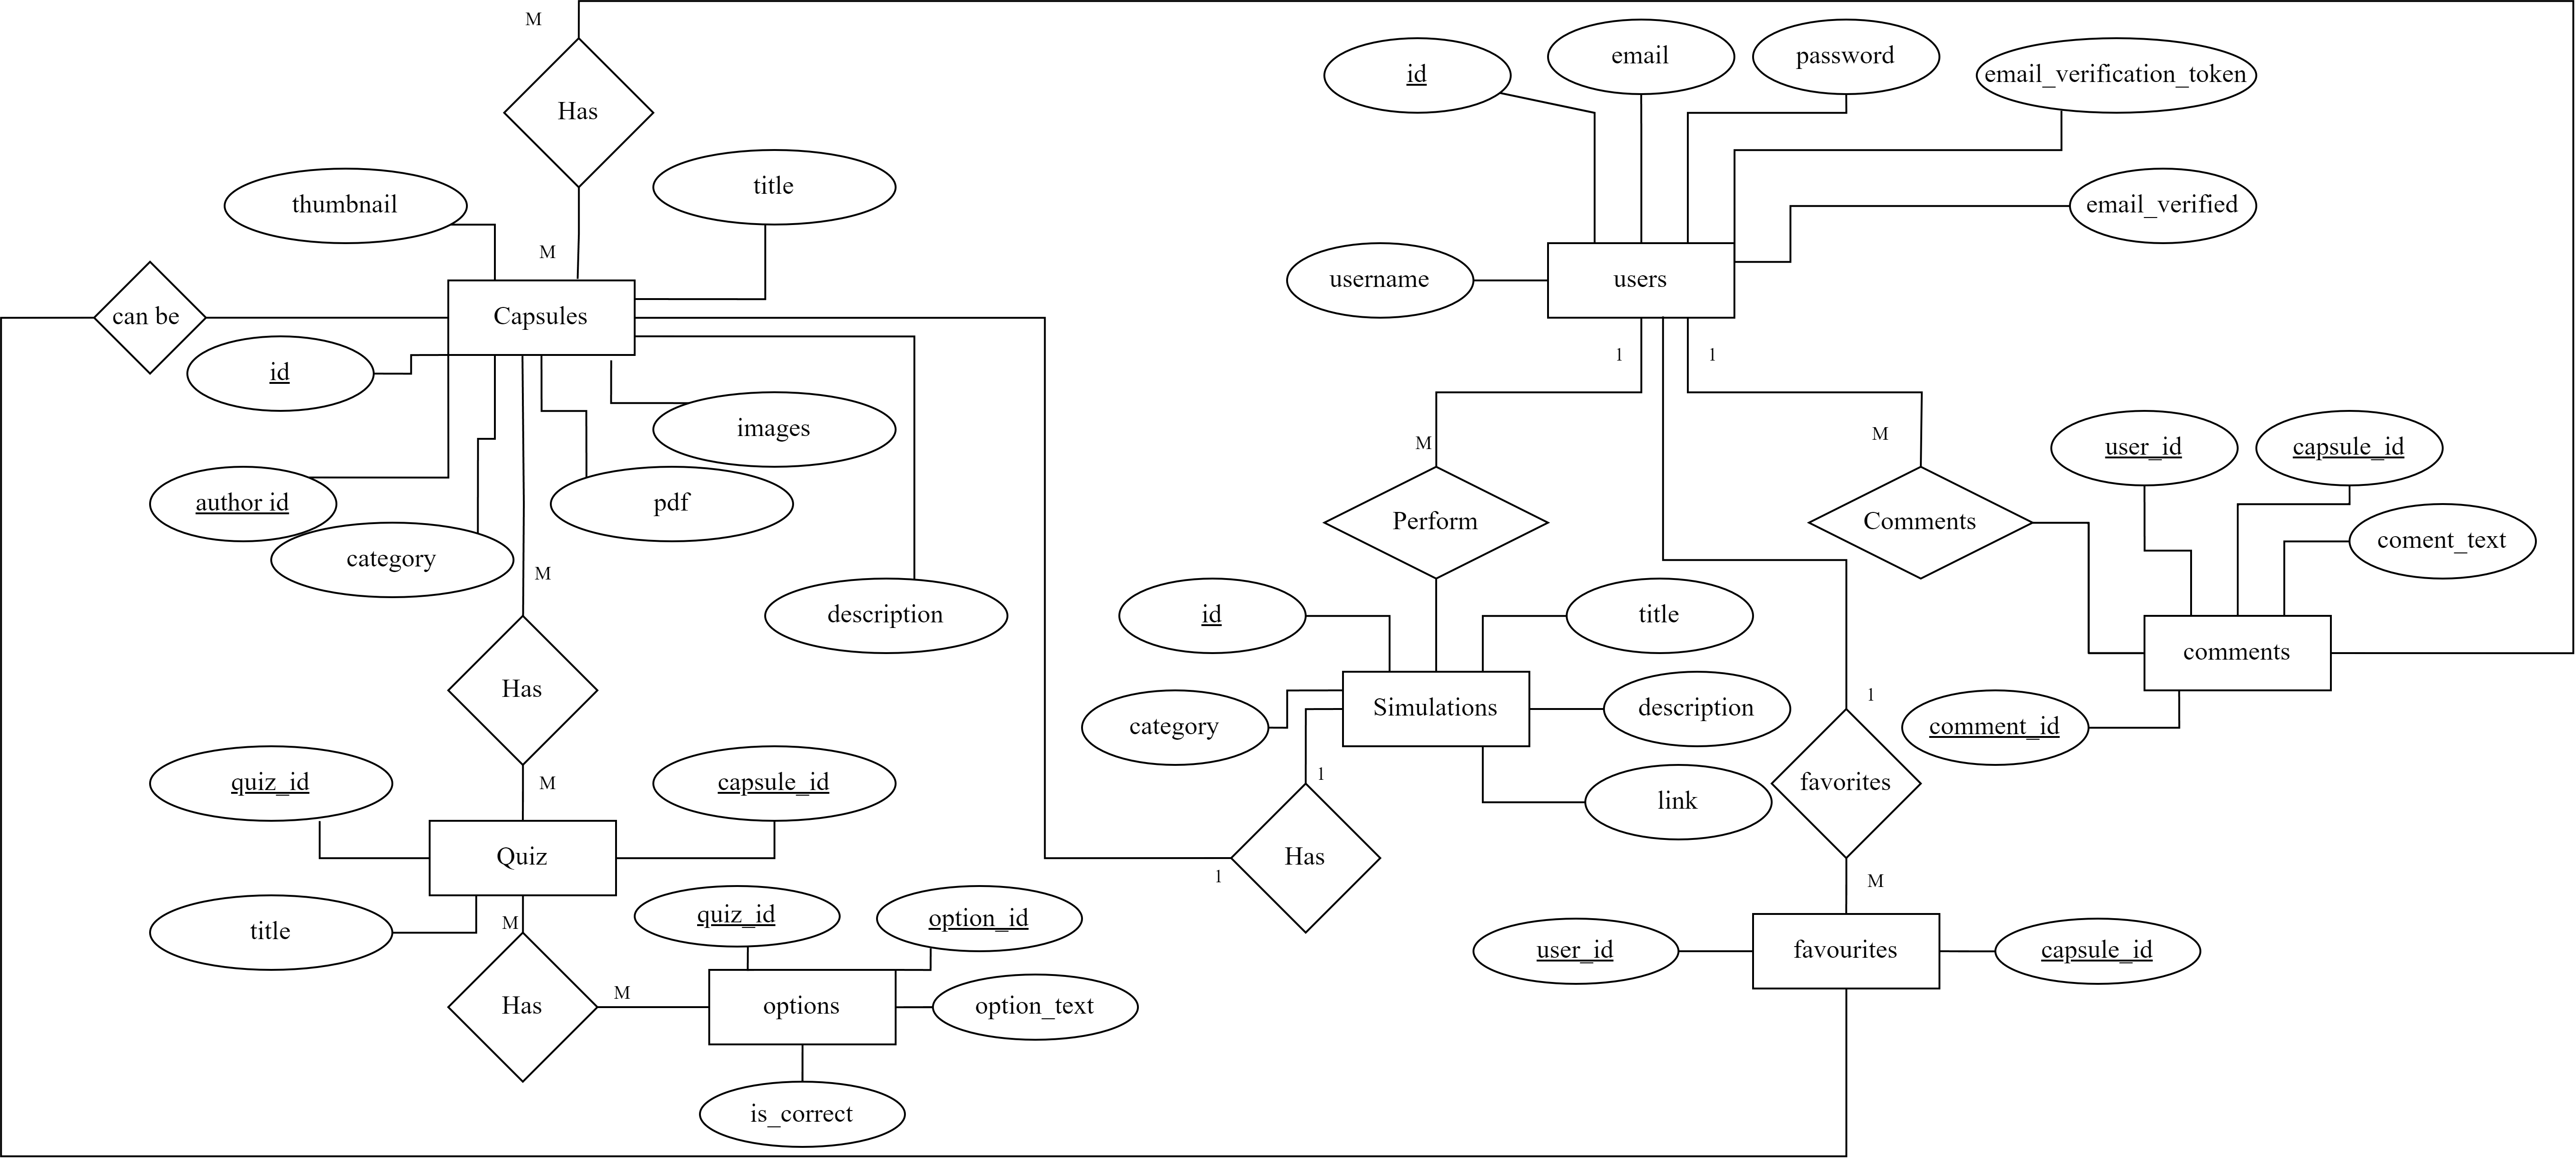
\includegraphics[height=10.5cm]{Diagrams/er.drawio.png}
    }
    \caption{ER Diagram of System Data}
\end{figure}
\newpage
\section{Structured System Design}
\subsection{Architecture Design}
The following diagram illustrates the architecture of our application. The application is structured using a three-tier architecture to ensure a clear separation of concerns and efficient functionality. The Presentation Layer, built with React.js, manages the user interface and user interactions. The Business Logic Layer, developed with Node.js and Express, handles core operations through middleware, routes, models, controllers, and utilities. Finally, the Data Management Layer uses PostgreSQL for relational database management and local server storage for handling files.
\begin{figure}[H]
    \centering
    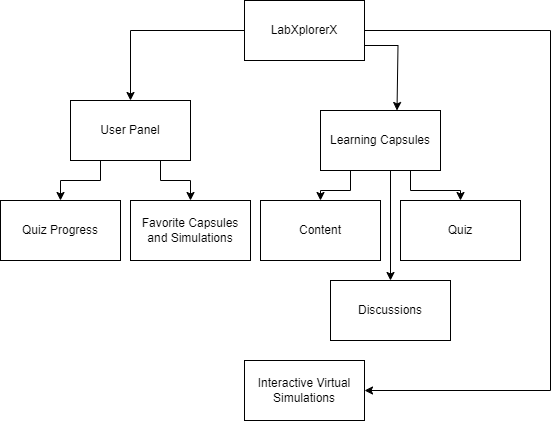
\includegraphics[height=16cm]{Diagrams/Main_Block.png}
    \caption{Three Tier Architecture of System}
\end{figure}

\newpage
\subsection{Database Schema Design}
The schema design details the tables, their attributes, and the relationships between them, ensuring that data is stored efficiently and consistently. This design includes defining primary keys to uniquely identify records, foreign keys to establish relationships between tables, and constraints to maintain data integrity. The schema design provides a clear blueprint for creating and managing the database, supporting effective data organization and retrieval as per the application’s requirements.
\begin{figure}[H]
   \centering
    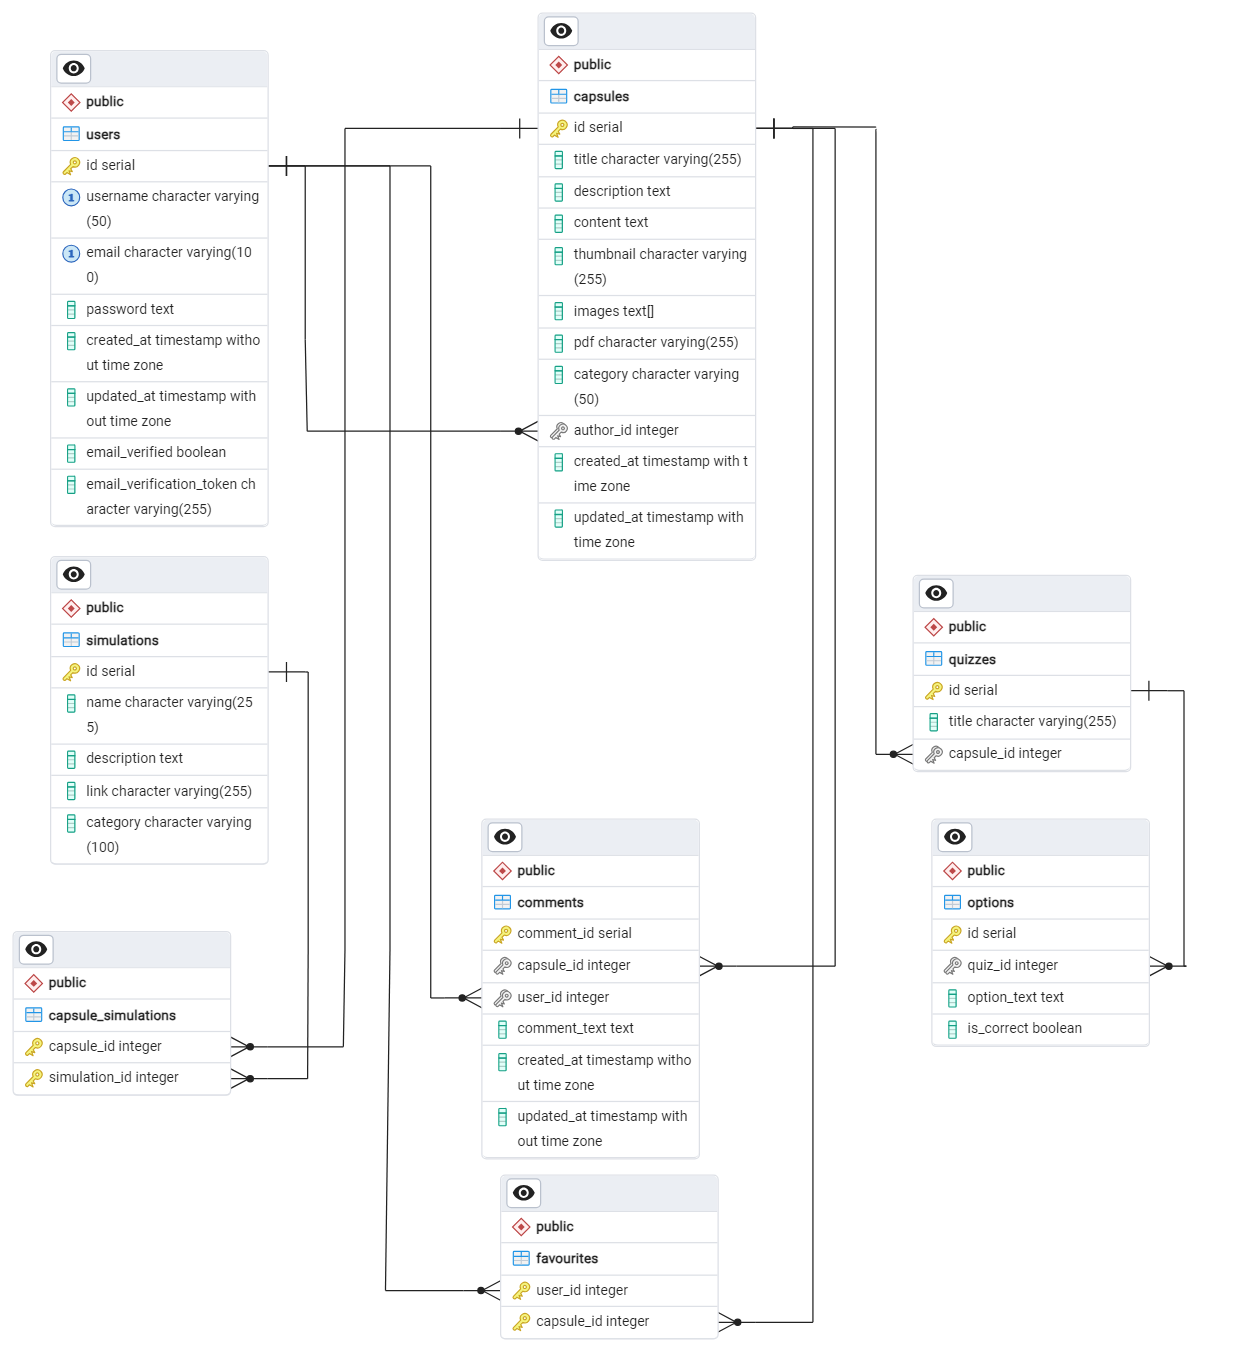
\includegraphics[height = 17cm]{Diagrams/Schema Design.png}
    \caption{Schema Design}
\end{figure}
\newpage

\subsection{Interface Design}
The interface design for this project focuses on creating a visually appealing, functional, and accessible user experience. The designs include layouts for the Home Screen, Menu, Capsule, Profile, and Admin Dashboard. Below is a detailed summary of the key design components:

\begin{itemize} 
    \item \textbf{Main Theme Color : Slate} The primary color used across the interface is Slate, chosen for its calm and professional appearance. This provides a consistent visual identity throughout the application while ensuring readability and contrast with other UI elements. 
    \item \textbf{Font : Poppins} The Poppins font is selected for its modern and clean look. It enhances the readability of text across all devices, providing a uniform typographic structure that complements the design's minimalistic approach.
    \item \textbf{Button Colors:}  
    Buttons are designed using a palette of Slate, Red, Green, and Blue. The different colors are used to signify various actions:  
    \begin{itemize}
        \item \textit{Slate:} Default or secondary actions
        \item \textit{Red:} Alerts or destructive actions (e.g., delete)
        \item \textit{Green:} Confirmation or positive actions (e.g., submit)
        \item \textit{Blue:} Primary actions (e.g., next, save)
    \end{itemize}
    \item \textbf{Accessibility Design:} The interface follows accessibility best practices by incorporating clearly defined and large buttons. These are designed to be easily distinguishable for users with visual impairments or motor difficulties, promoting ease of use.
     \item \textbf{Responsive Design:} While the UI components have been optimized for responsiveness across different devices, the simulations are not responsive. The focus is on ensuring that primary UI elements scale effectively for various screen sizes, maintaining usability and aesthetics.
    \item \textbf{Button Design:} Buttons throughout the interface are designed to be large and easily clickable. Their size and prominence ensure effortless navigation, reducing the chance of misclicks, and enhancing the overall user experience for a broad range of users.
    \item \textbf{Form Design:} The form design prioritizes clarity, validation, and accessibility. Below are the key design considerations:
     \begin{itemize}
        \item \textbf{Clear Labels and Placeholders:} 
        All form fields are accompanied by clear labels and visible placeholders, ensuring that users can easily understand the required input.
        
        \item \textbf{Validation Feedback:} 
        Real-time validation is implemented to give users immediate feedback. 
        
        \item \textbf{Keyboard Navigation:} 
        The form is designed to support keyboard navigation, allowing users to efficiently move through fields using the tab key. This feature improves accessibility for users who rely on keyboards or other assistive devices to interact with the form.
    \end{itemize}
    
\end{itemize}
\textbf{UI Designs}
\begin{figure}[H]
   \centering
    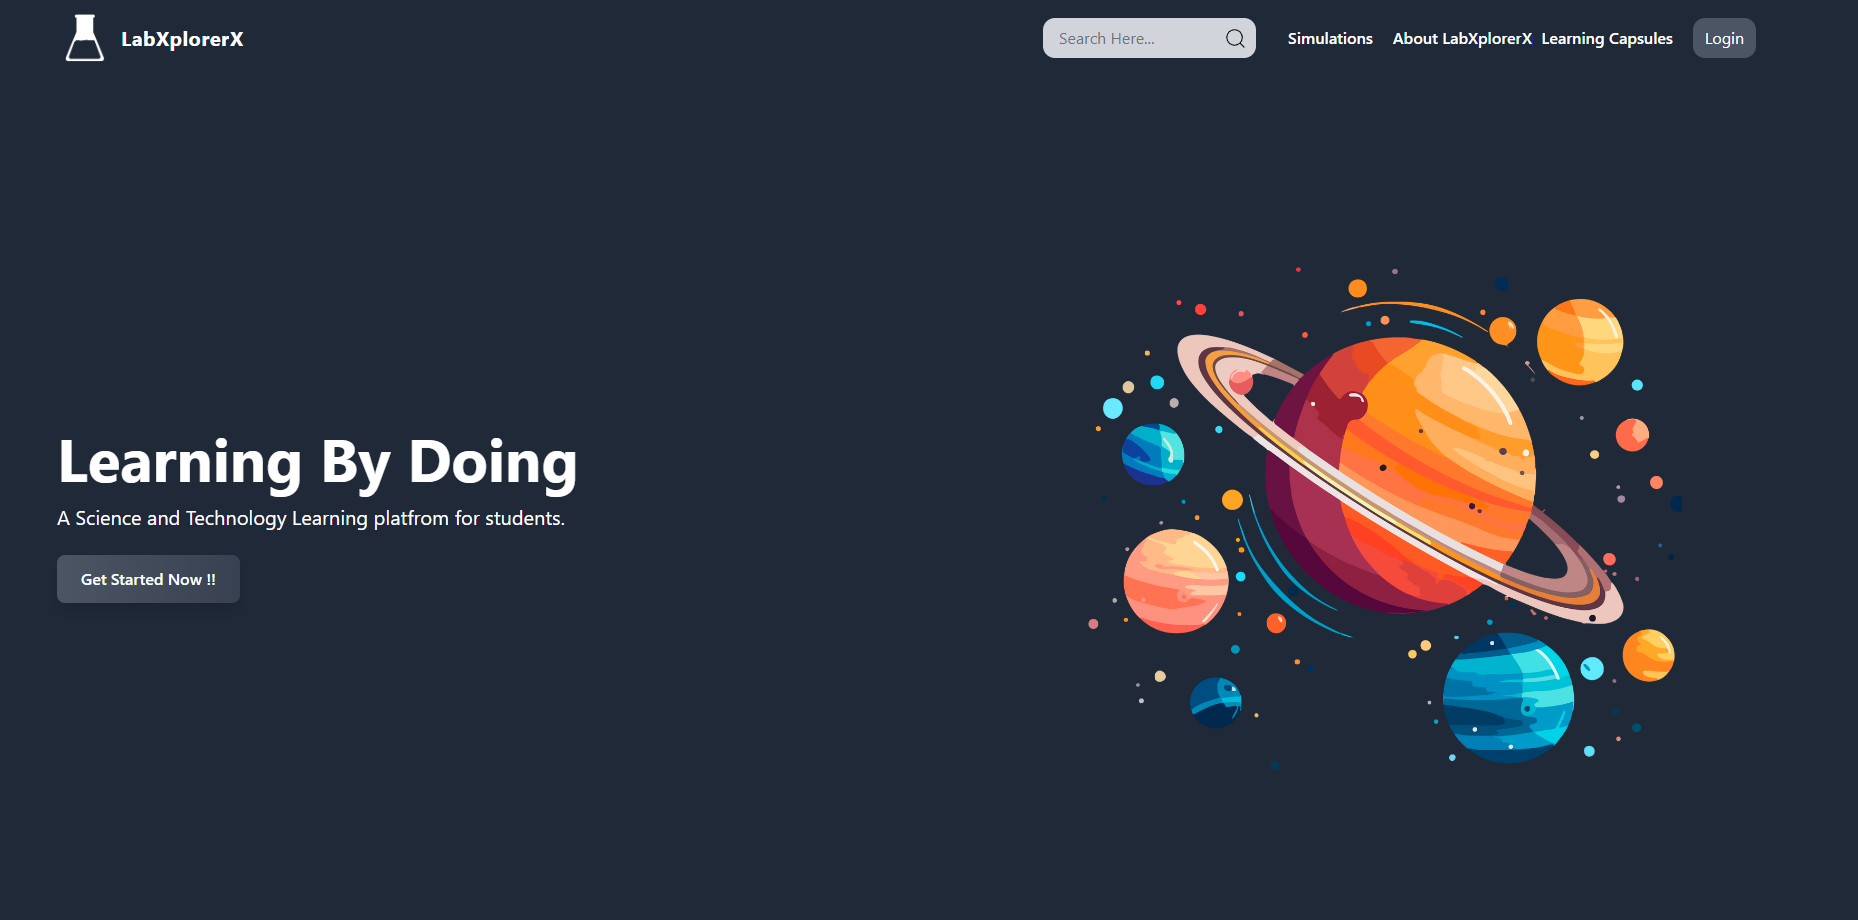
\includegraphics[width = 15cm]{Diagrams/interface/home ui.png}
    \caption{Home Screen UI Design}
\end{figure}
\begin{figure}[H]
    \centering
     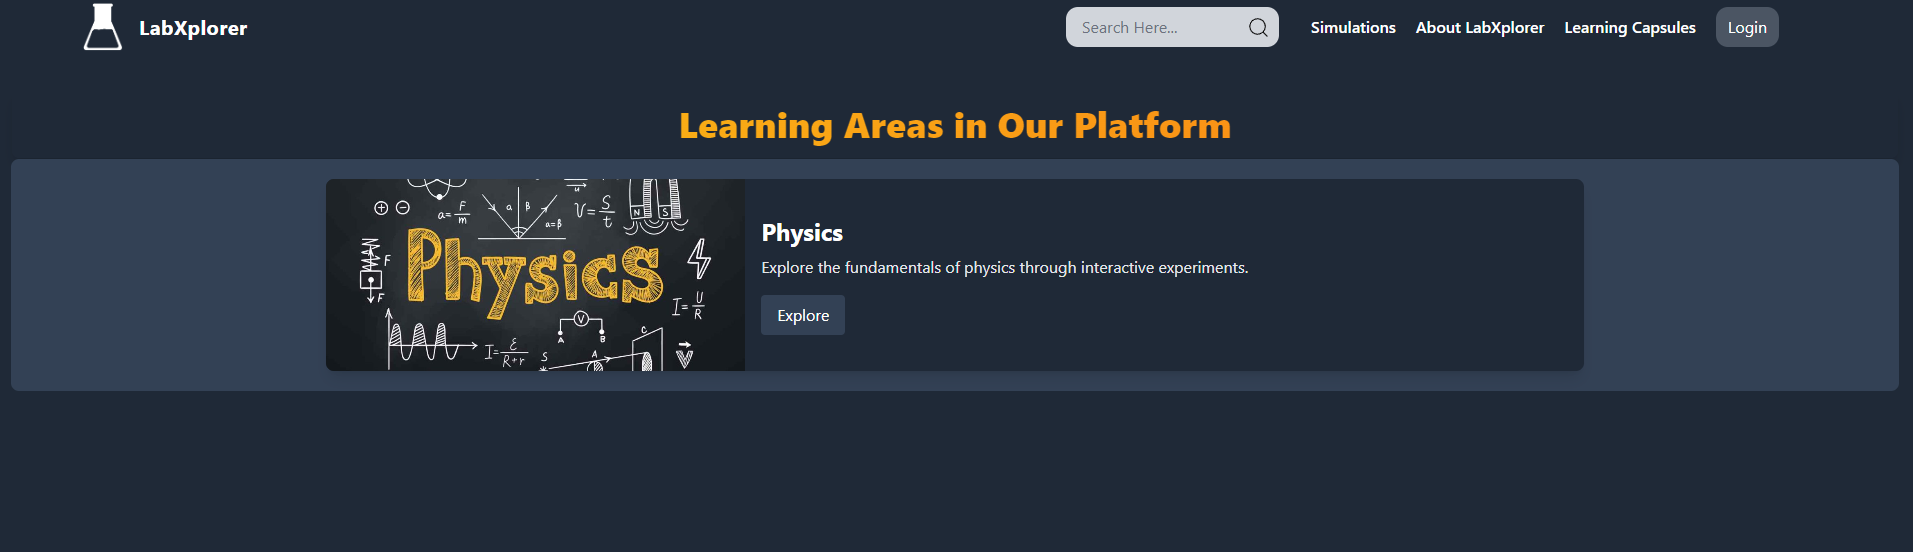
\includegraphics[width = 15cm]{Diagrams/interface/capsule category ui.png}
     \caption{Capsule Category UI Design}
 \end{figure}
 \begin{figure}[H]
    \centering
     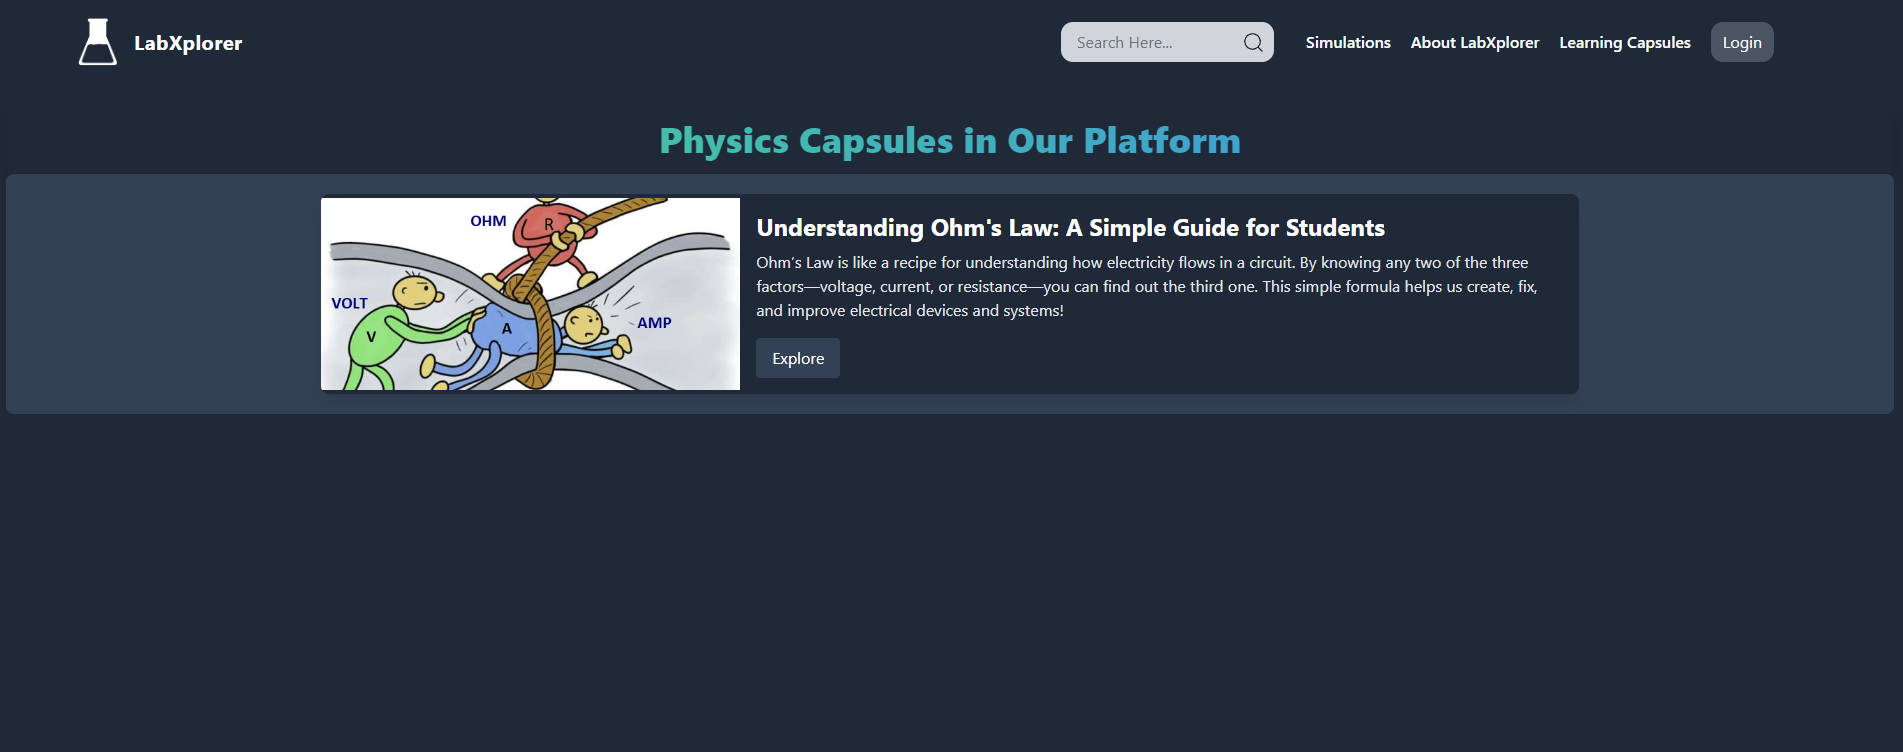
\includegraphics[width = 15cm]{Diagrams/interface/Capsules.png}
     \caption{Capsules Menu Design}
 \end{figure}
 \begin{figure}[H]
    \centering
     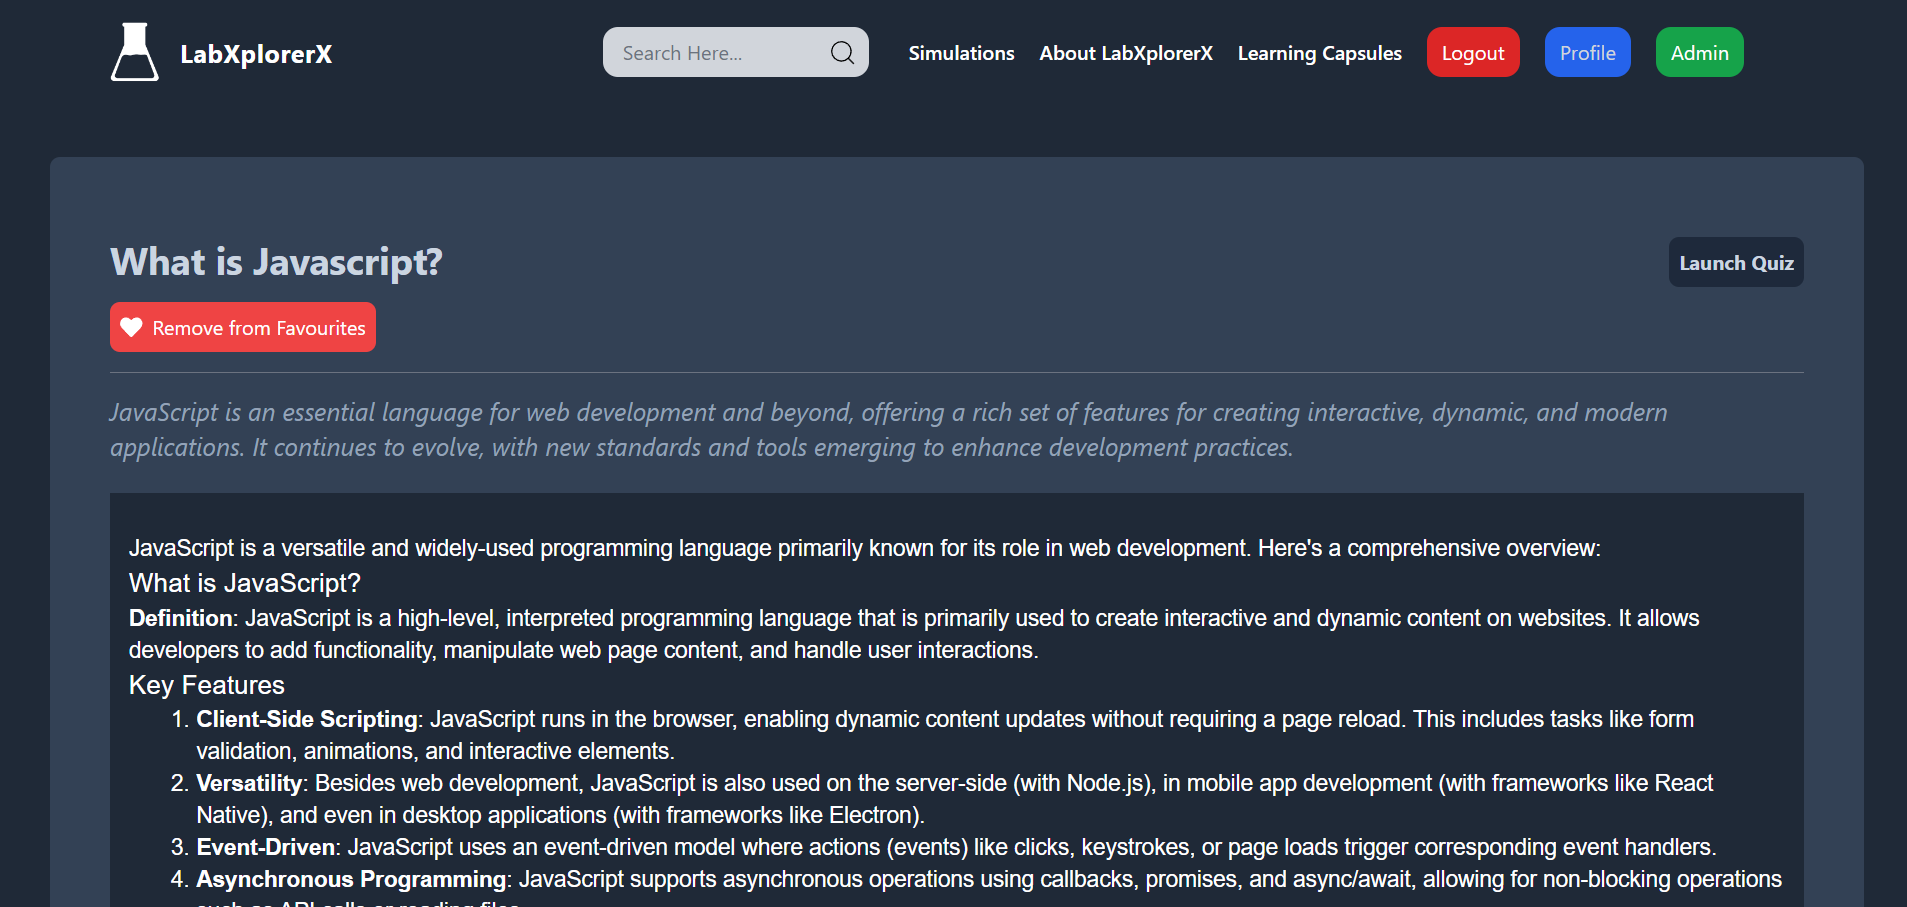
\includegraphics[width = 15cm]{Diagrams/interface/cap.png}
     \caption{Capsules Menu Design}
 \end{figure}
 \begin{figure}[H]
    \centering
     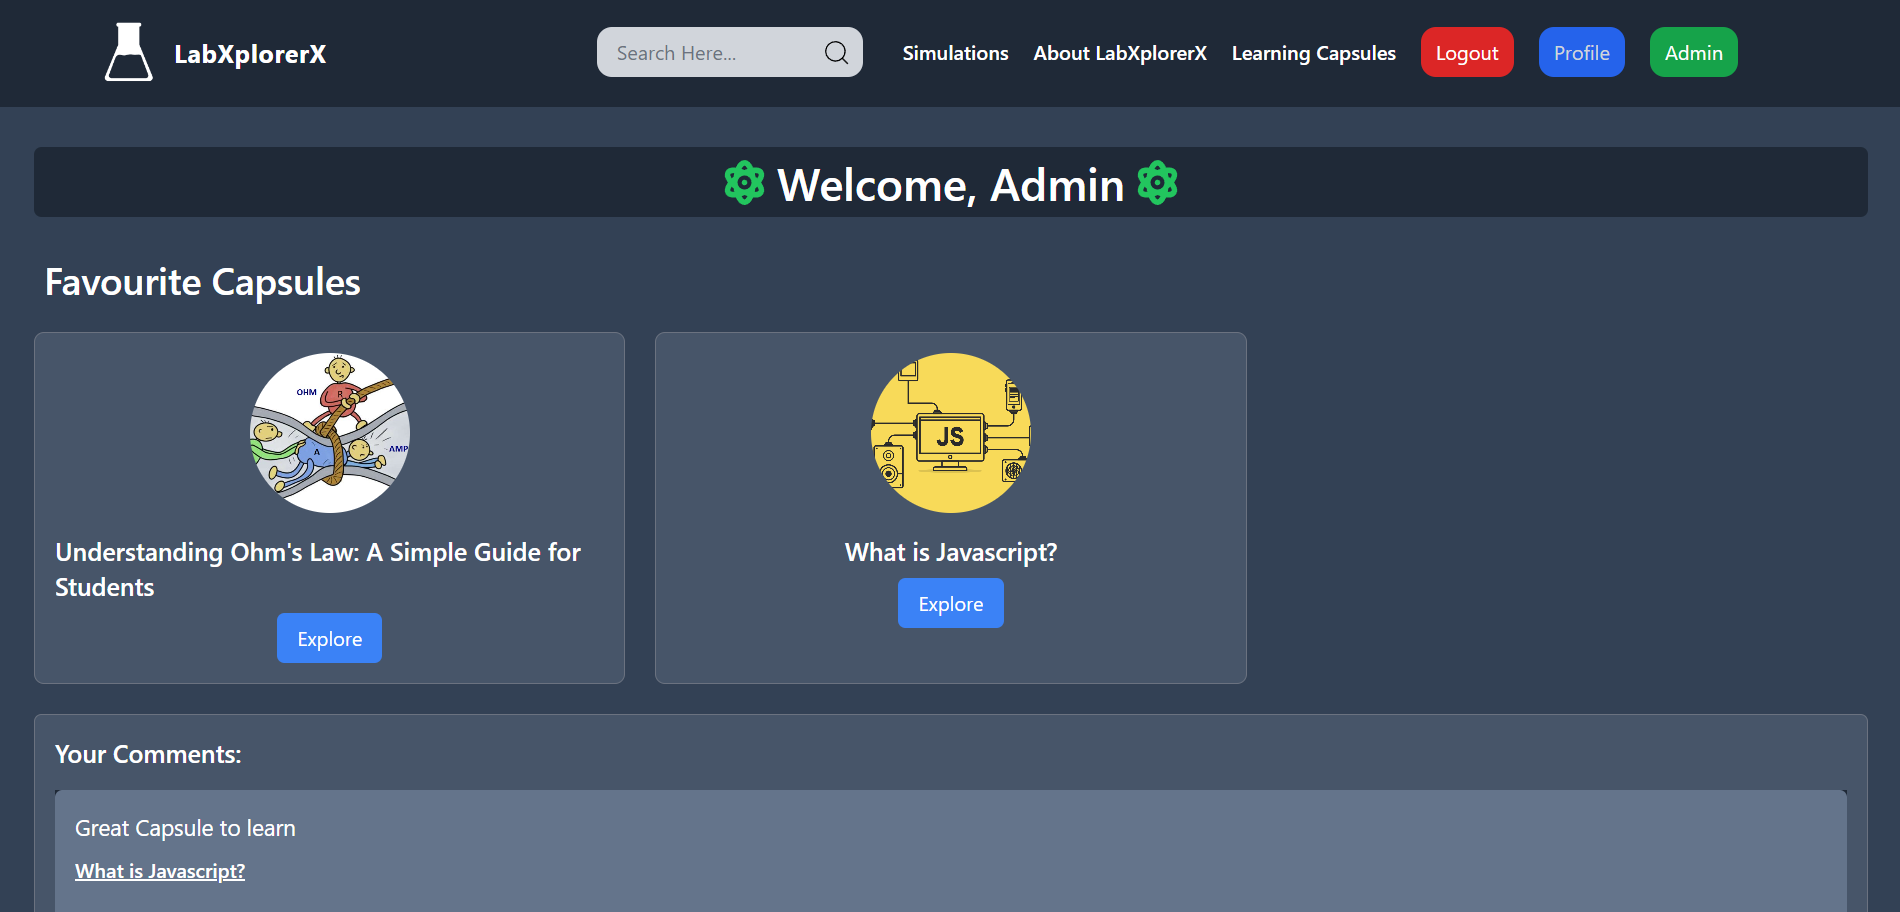
\includegraphics[width = 15cm]{Diagrams/interface/admin.png}
     \caption{Capsules Menu Design}
 \end{figure}
 \begin{figure}[H]
    \centering
     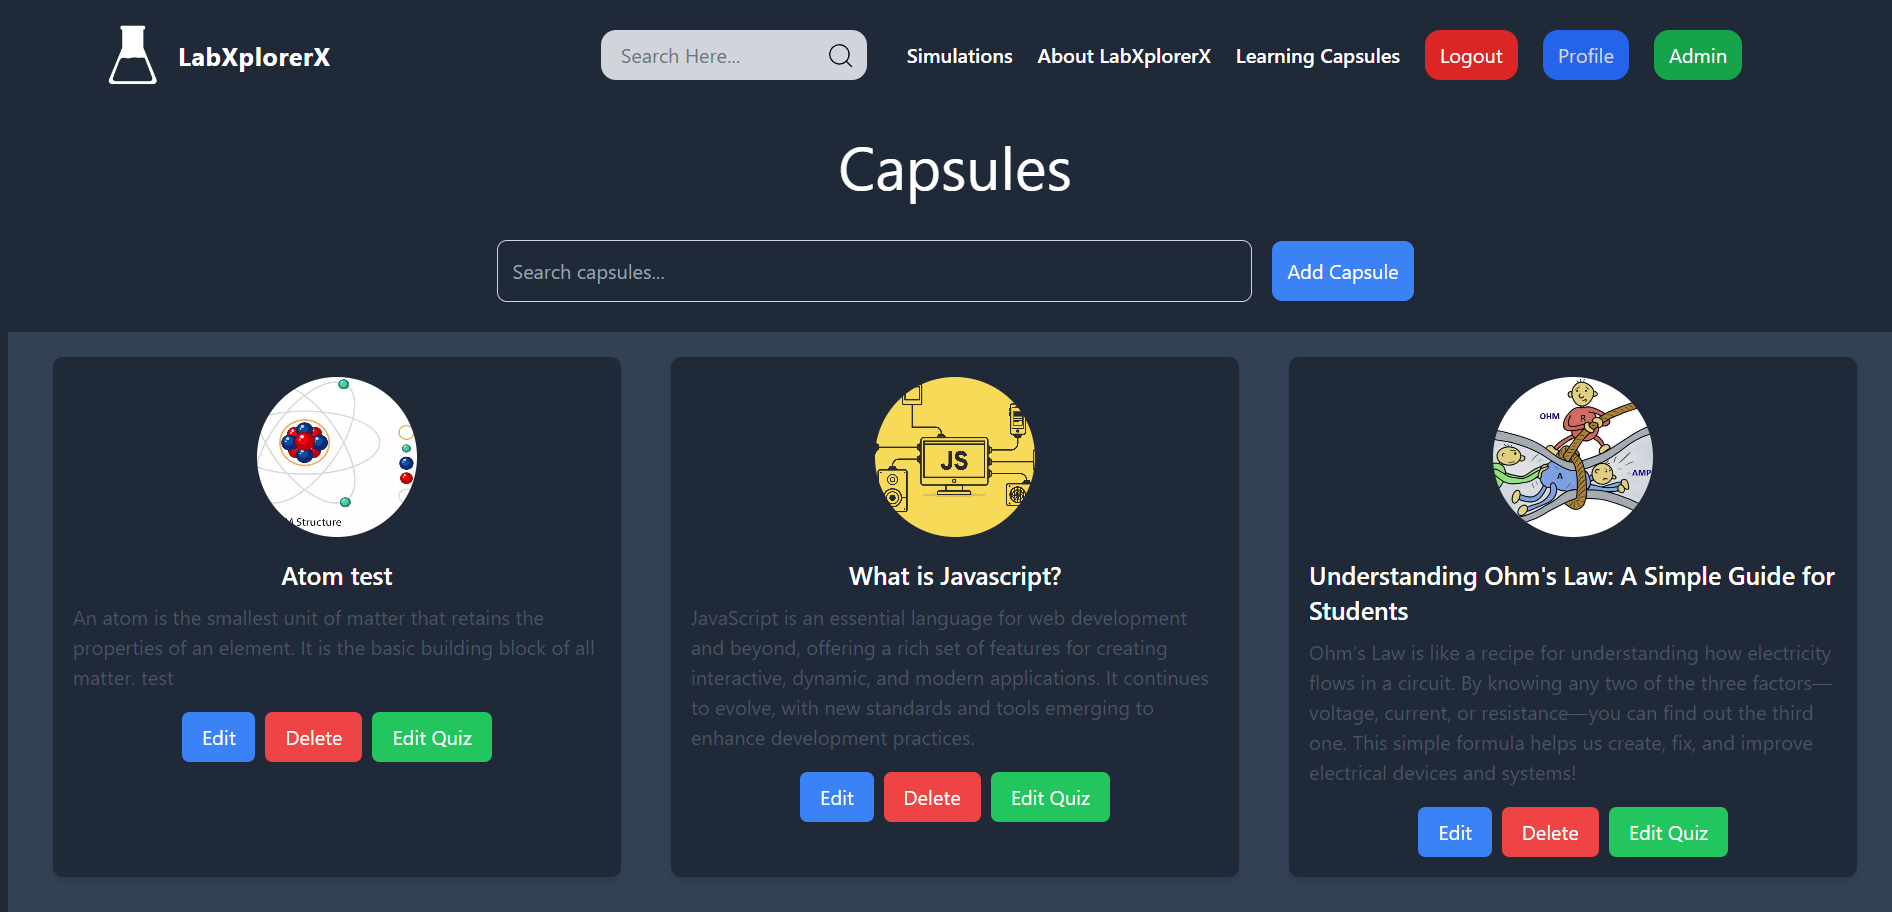
\includegraphics[width = 15cm]{Diagrams/interface/admin_dash.png}
     \caption{Capsules Menu Design}
 \end{figure}
 \begin{figure}[H]
    \centering
     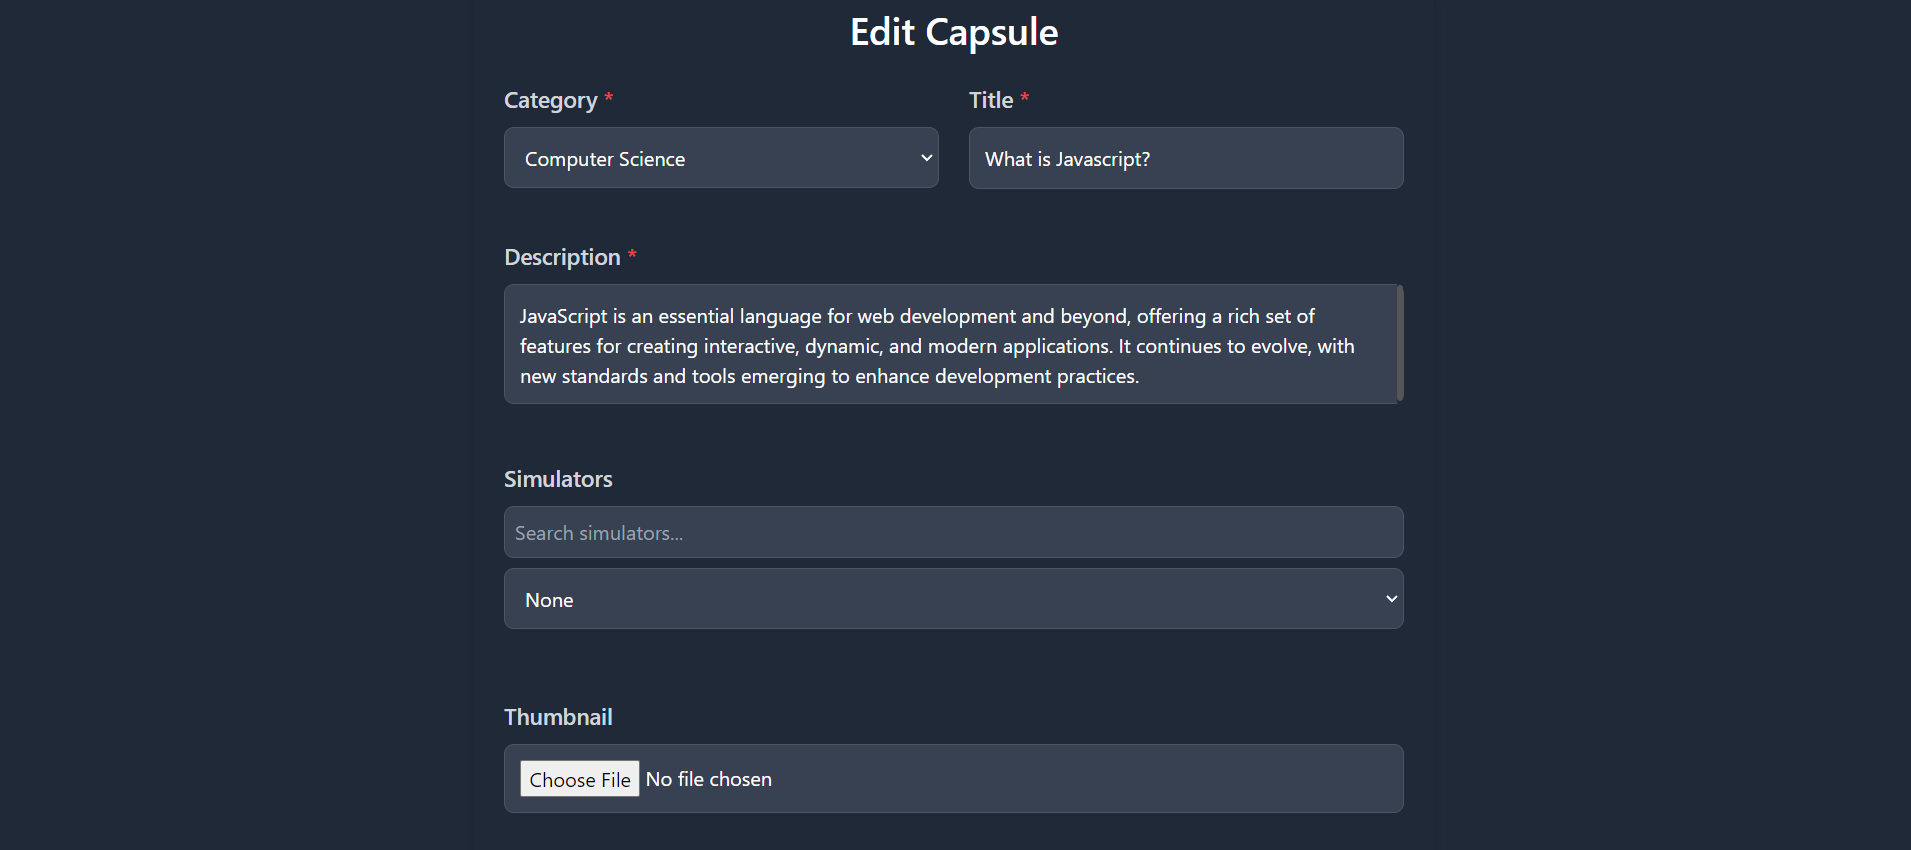
\includegraphics[width = 15cm]{Diagrams/interface/edit.png}
     \caption{Capsules Menu Design}
 \end{figure}
\newpage
\subsection{Physical DFD}
This Physical Data Flow Diagram (DFD) outlines the architecture of a web application with a clear separation of frontend and backend components. On the backend, Express (Node.js) handles the server-side logic, with middleware for authentication and error handling, routes for user, admin, and capsules, asynchronous controllers for managing requests, and a PostgreSQL database for storing data. Static files, including Unity simulations, are served from the backend. The frontend is built with React.js, utilizing React Router for navigation and RTK slices and APIs for state management. Screens and UI components, along with Phaser simulations, allow users to interact with backend data and display both static and dynamic simulations. The central store handles state management locally across components.
\begin{figure}[H]
    \centering
    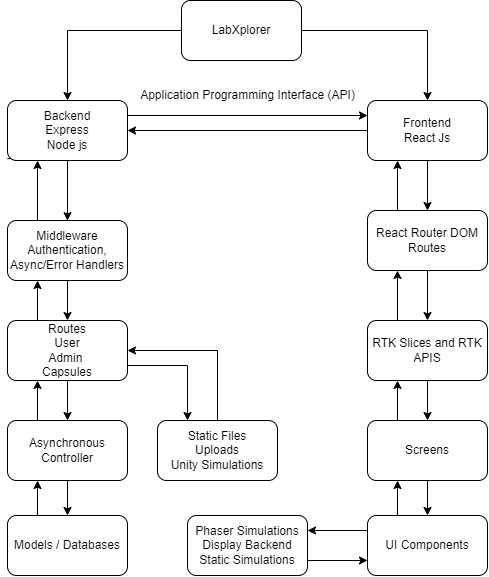
\includegraphics[height = 15cm]{Diagrams/DFD Process Modeling.png}
    \caption{Physical Data Flow Diagram}
\end{figure}
\newpage
\chapter{ALGORITHMS}

\section{Algorithm of AtomSimulator}
Atom Sim is a virtual lab simulation tool designed to provide an interactive and educational experience in understanding atomic and molecular structures.
\begin{itemize}
    \item \textbf{Initialization:} Initializes \texttt{selectedElement} with the first element from the \texttt{elements} array.
    \item \textbf{Game Setup:} Configures and initializes a Phaser game instance with specified dimensions and physics.
    \item \textbf{Atom Visualization:} Creates a nucleus and displays protons and neutrons; draws electron orbits and positions electrons in their respective orbits.
    \item \textbf{Electron Movement:} Uses a timer event to update electron positions based on their orbits and the current time.
    \item \textbf{User Interaction:} Updates \texttt{selectedElement} and re-renders the game scene when a new element is selected.
    \item \textbf{Cleanup:} Destroys the Phaser game instance when the component unmounts to free up resources.
\end{itemize}


\section{Algorithm of CodeEditor}
The `CodeEditor` component allows users to write, run, and view JavaScript code in a simulated environment.
\begin{itemize}
    \item \textbf{Initialization:} Sets initial states for `code` (user input) and `consoleOutput` (output from the iframe).
    \item \textbf{Event Handling:} Listens for messages from the iframe to capture console output and errors.
    \item \textbf{Code Execution:} Creates an iframe to run the user-provided code, capturing and redirecting console messages.
    \item \textbf{User Interaction:} Updates the `consoleOutput` based on the iframe’s console messages and renders the results.
    \item \textbf{Cleanup:} Removes the iframe from the DOM after execution to prevent resource leaks.
\end{itemize}
\section{Algorithm of OhmsLawSimulator}
The `OhmsLawSimulator` component simulates Ohm's Law, allowing users to interactively adjust voltage and resistance to observe their effects.
\begin{itemize}
    \item \textbf{Initialization:} Sets default values for voltage and resistance. Initializes Phaser game instance and scene references.
    \item \textbf{Game Setup:} Configures and starts a Phaser game with physics and rendering settings. Preloads assets and creates initial game elements like a static rectangle and a dynamic bulb.
    \item \textbf{Simulation Update:} Continuously updates bulb brightness based on the calculated current (using Ohm's Law: \( I = \frac{V}{R} \)). Adjusts displayed values for voltage, resistance, and current.
    \item \textbf{User Interaction:} Updates Phaser scene values directly when voltage or resistance inputs change, triggering a re-render of the simulation.
    \item \textbf{Cleanup:} Destroys the Phaser game instance when the component unmounts to free up resources.
\end{itemize}
\section{Algorithm of GravitySim}
The `GravitySim` component simulates gravity effects on a player sprite, providing interactive controls for adjusting gravity and managing the simulation.
\begin{itemize}
    \item \textbf{Initialization:} Sets up a Phaser game instance with a gravity simulation environment. Initializes references for the game, player, text elements, and timer.
    \item \textbf{Game Setup:} Loads assets, creates game elements (background, platforms, and player), and displays initial values for gravity, distance, and time. Pauses the simulation and player's movement initially.
    \item \textbf{Simulation Update:} Continuously updates gravity text, distance traveled, and elapsed time. Adjusts text position relative to the player sprite and handles the timer based on simulation state (paused or running).
    \item \textbf{User Interaction:} Provides buttons for increasing/decreasing gravity, resetting player position, pausing, and resuming the simulation. Updates the game state and UI accordingly.
    \item \textbf{Cleanup:} Destroys the Phaser game instance when the component unmounts to release resources.
\end{itemize}
\textbf{Key Formula:}\\
The distance traveled by the player due to gravity can be approximated using the formula for free-fall motion:
\[
d = \frac{1}{2} g t^2
\]
where:
\begin{itemize}
    \item \(d\) is the distance traveled (in meters),
    \item \(g\) is the acceleration due to gravity (in meters per second squared),
    \item \(t\) is the time elapsed (in seconds).
\end{itemize}
In the simulation, this formula is used to calculate and display the distance the player has fallen based on the current gravity setting and elapsed time.
\section{Algorithm for SolarSystemSimulator}

\begin{enumerate}
    \item \textbf{Initialization:}
    \begin{itemize}
        \item Define celestial bodies (Sun, planets, moons) as GameObjects.
        \item Set up the main camera.
    \end{itemize}
    
    \item \textbf{Setup Rotation:}
    \begin{itemize}
        \item Attach \texttt{RotateAround} script to celestial bodies.
        \item Set rotation targets (e.g., planets orbit around Sun, moons around planets).
        \item Use \texttt{transform.RotateAround} for rotation.
    \end{itemize}
    
    \item \textbf{Camera Behavior:}
    \begin{itemize}
        \item Attach \texttt{FollowAtTarget} script to the main camera.
        \item Update camera to \texttt{LookAt} the target.
    \end{itemize}
    
    \item \textbf{User Interaction:}
    \begin{itemize}
        \item Attach \texttt{ChangeLookAtTarget} script to celestial bodies.
        \item On click, update camera target and adjust \texttt{fieldOfView}.
    \end{itemize}
    
    \item \textbf{Implementation Steps:}
    \begin{itemize}
        \item Create celestial bodies and attach scripts.
        \item Configure camera controls.
        \item Test rotation, camera focus, and user interactions.
    \end{itemize}
    
\end{enumerate}


% \section{Algorithm Details}